%%%%%%%%%%%%%%%%%%%%%%%%%%%%%%%%%%%%%%%%%%%%%%%%%%%%%%%%%%%%%%%%%%%%%%%%%%%%%
%
% Vorlage für Seminararbeiten im Institut für Verteilte Systeme
% 
% HINWEISE
% 
%  1. Bei Nutzung für Seminarausarbeitungen darf insbesondere die Schriftart
%     und -größe nicht angepasst werden.
%  2. Die Vorlage unterstützt deutsche und englische Ausarbeitungen durch
%     Anpassung der babel Paketoptionen.
%  3. Folgende Angaben sollen angepasst werden:
%     - Titel der Arbeit
%     - Name und E-Mail-Adresse des Autors
%     - Titel des Seminars
%     - Semester
%  4. Die Vorlage sieht eine Lizensierung unter CC-BY-SA vor, die jedoch
%     nicht verpflichtend ist. Falls nicht gewünscht, bitte alle \thanks
%     Befehle auskommentieren.
%     Die gewählte Lizenz (CC-BY-SA) ist kompatibel mit einer möglichen
%     Veröffentlichung auf dem Volltextserver der Uni Ulm
%     (http://vts.uni-ulm.de).
%
%%%%%%%%%%%%%%%%%%%%%%%%%%%%%%%%%%%%%%%%%%%%%%%%%%%%%%%%%%%%%%%%%%%%%%%%%%%%%

% Based on the IEEE Journal style.
\documentclass[10pt,a4paper,compsoc,peer review papers]{IEEEtran}

\usepackage{graphicx}
\usepackage[cmex10]{amsmath}
\usepackage[ngerman]{babel} % Deutsche Ausarbeitung
% \usepackage[USenglish]{babel} % Englische Ausarbeitung
\usepackage{url}
\usepackage[colorlinks]{hyperref}
\usepackage{color}  % Definition von Linkfarben
\definecolor{DarkRed}{rgb}{0.5,0,0}
\hypersetup{
  colorlinks,
  citecolor=DarkRed,
  linkcolor=DarkRed,
  urlcolor=blue}
\usepackage[utf8]{inputenc}
\usepackage[T1]{fontenc}  % Korrekte Umlaute im Output

\newcommand\IEEEfirstsection[1]{%
  \noindent\raisebox{2\baselineskip}[0pt][0pt]%
  {\parbox{\columnwidth}{#1%
  \global\everypar=\everypar}}%
  \vspace{-1\baselineskip}\vspace{-\parskip}\par
}

\newcommand\cclicense{{\normalfont\sffamily\bfseries CC-BY-SA}}
\IfFileExists{ccicons.sty}{%
\usepackage{ccicons}
\renewcommand\cclicense{\ccbysa}
}

\begin{document}

\title{LEX 2016: Bestimmung der Wolkenhöhe mittels Pyrgeometer}

\author{%
\IEEEauthorblockN{Lukas Kluft}\\
\IEEEauthorblockA{\url{lukas.kluft@gmail.com}}%
%
%\iflanguage{ngerman}{%
%\thanks{%
%\cclicense{}
%Diese Arbeit steht unter einer
%Creative Commons Namensnennung - Weitergabe unter gleichen Bedingungen
%3.0 Deutschland Lizenz.}%
%\thanks{\url{http://creativecommons.org/licenses/by-sa/3.0/de/}}%
%}{ % Englische Ausarbeitung
%\thanks{%
%\cclicense{}
%This work is licensed under a
%Creative Commons Attribution-ShareAlike 4.0 International License.}%
%\thanks{\url{http://creativecommons.org/licenses/by-sa/4.0/}}%
%}%
}

\IEEEpubid{\sffamily%
\makebox[\columnwidth]{\hfill Lehrexkursion Fehmarn}%
\makebox[\columnsep]{$\cdot$}%
\makebox[\columnwidth]{SS 2016,
Meteorologisches Institut - CEN, Universit"at Hamburg\hfill}}

\IEEEtitleabstractindextext{%
\begin{abstract}
Pyrgeometer messen die aus dem Halbraum eintreffende atmosphärische
Gegenstrahlung (5-50\,$\mu$m). Die Stärke der Gegenstrahlung hängt vom
Zustand der Atmosphäre ab; bei Bewölkung ist diese deutlich stärker als bei
wolkenfreien Verhältnissen. Zusätzlich hängt die Emission von der Temperatur
ab; warme Körper strahlen stärker als kalte. Diese beiden Effekte ermöglichen 
es über die atmosphärische Gegenstrahlung Rückschlüsse auf die Temperatur der
Wolkenunterkante zu ziehen. Mit Hilfe zusätzlicher Annahmen über das
Temperaturprofil kann so die Höhe der Wolkenunterkante abgeschätzt werden.
\end{abstract}%
}

\maketitle

\IEEEfirstsection{\section{Grundlagen}\label{sec:grundlagen}}


\section{Strahlungstransfer}\label{sec:strahlungstransfer}
Pyrgeometer messen den gesamten Strahlungsfluss im langwelligen
Frequenzspektrum zwischen 3\,THz und 60\,THz. Um genauere Informationen darüber
zu gewinnen, aus welchen Teilen der Atmosphäre die gemessene Strahlung stammt,
wurden Strahlungstransferrechnungen durchgeführt.

Für die Berechnung wurde der Atmospheric Radiative Transfer Simulator (ARTS)
verwendet \cite{Eriksson2011}. ARTS ist ein physikalisches
Strahlungstransfermodell für den Millimeter- und Submillimeterbereich des
elektromagnetischen Strahlungsspektrums.


\section{Messungen}\label{sec:messungen}

\subsection{Pyrgeoemter}\label{subsec:pyrgeometer}

% TODO: find out which thermometer is used.
\subsection{Thermometer}\label{subsecthermometer}

\subsection{Ceilometer}\label{subsec:ceilomter}


\section{Ergebnisse}\label{sec:ergebnisse}
% \begin{figure}[ht]
%     \centering
%     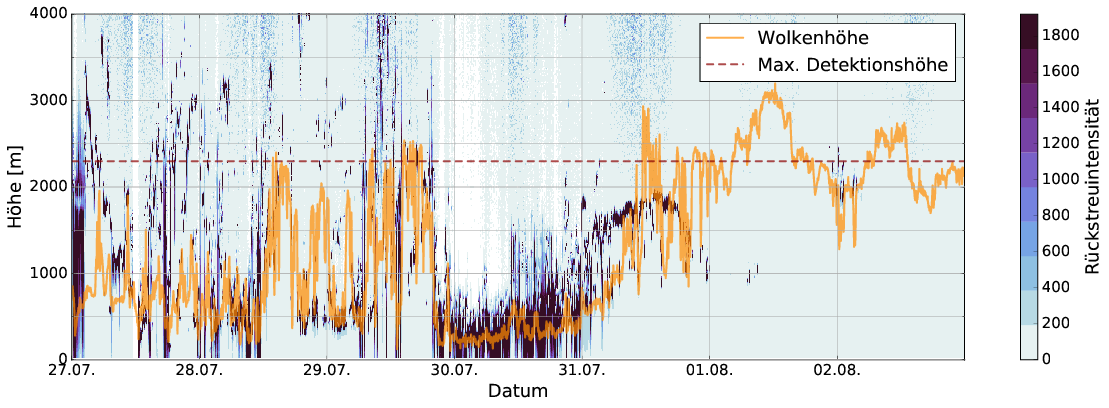
\includegraphics[width=0.48\textwidth]{figures/ceilometer.png}
%     \caption{Zeitreihe der Rückstreuintensität sowie der ermittelten Wolkenhöhe.}
%     \label{fig:back_scat}
% \end{figure}


\section{Schlussfolgerungen}\label{sec:schlussfolgerungen}

% bibliography
\bibliographystyle{IEEEtranS}
\bibliography{references}

\end{document}
